\title{Aula 13 - Firewalls}

\author{Prof. Gabriel Rodrigues Caldas de Aquino}

\institute
{
    Instituto de Computação \\
    Universidade Federal do Rio de Janeiro\\
    gabrielaquino@ic.ufrj.br% Your institution for the title page
}
\date{Compilado em: \\ \today} % Date, can be changed to a custom date

%----------------------------------------------------------------------------------------
%    PRESENTATION SLIDE
%----------------------------------------------------------------------------------------



\begin{frame}
    % Print the title page as the first slide
    \titlepage
\end{frame}

\begin{frame}{Firewalls e VPNs}


    \begin{figure}
        \centering
        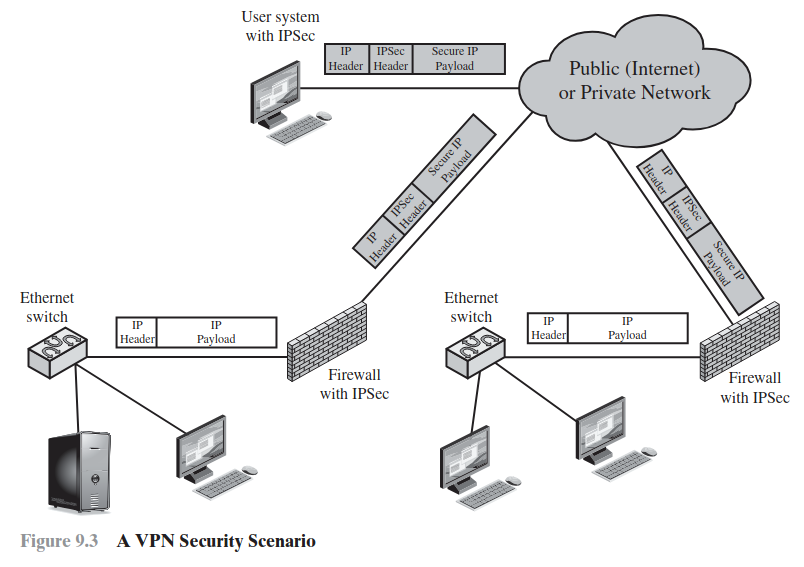
\includegraphics[width=0.7\textwidth]{Figuras/firewalls-vpns.png}


    \end{figure}

\end{frame}

\begin{frame}{O que são Firewalls}
    \begin{itemize}
        \item Firewalls são um meio \textbf{eficaz} de proteger um sistema local ou uma rede contra ameaças de segurança baseadas em rede.

        \item \textbf{O Dilema (O Balanço):}
              \begin{itemize}
                  \item \textbf{Proteger} os ativos internos contra ameaças.
                  \item Ao mesmo tempo, \textbf{permitir} o acesso ao mundo exterior (WANs e Internet).
              \end{itemize}

        \item \textbf{9.1 A Necessidade de Firewalls}
              \begin{itemize}
                  \item A necessidade de firewalls é resultado direto da \textbf{evolução} constante dos sistemas de informação em corporações, agências governamentais e outras organizações.
              \end{itemize}
    \end{itemize}
\end{frame}

\begin{frame}{A Necessidade de Firewalls: Evolução dos Sistemas (Parte 1)}
    \begin{itemize}
        \item Desenvolvimentos notáveis na evolução dos sistemas:

        \item \textbf{1. Sistema Centralizado (Mainframe)}
              \begin{itemize}
                  \item Um mainframe central suportando terminais diretamente conectados.
              \end{itemize}

        \item \textbf{2. Redes Locais (LANs)}
              \begin{itemize}
                  \item Interconectando PCs e terminais entre si e ao mainframe.
              \end{itemize}

        \item \textbf{3. Rede Local Corporativa (Premises Network)}
              \begin{itemize}
                  \item Consiste em várias LANs, interconectando PCs, servidores e (talvez) mainframes.
              \end{itemize}
    \end{itemize}
\end{frame}

\begin{frame}{A Necessidade de Firewalls: Evolução dos Sistemas (Parte 2)}
    \begin{itemize}
        \item Desenvolvimentos notáveis (continuação):

        \item \textbf{4. Rede Corporativa Ampla (Enterprise-wide)}
              \begin{itemize}
                  \item Múltiplas redes locais (premises) geograficamente distribuídas.
                  \item Interconectadas por uma \textbf{WAN privada}.
              \end{itemize}

        \item \textbf{5. Conectividade com a Internet}
              \begin{itemize}
                  \item As várias redes locais (premises) se conectam à Internet (além da WAN privada).
              \end{itemize}

        \item \textbf{6. Computação em Nuvem (Enterprise Cloud)}
              \begin{itemize}
                  \item Servidores virtualizados em data centers.
                  \item Provendo serviços internos (organizacionais) e externos (acessíveis pela Internet).
              \end{itemize}
    \end{itemize}
\end{frame}

\begin{frame}{O Dilema da Conectividade com a Internet}
    \begin{itemize}
        \item \textbf{A Realidade Atual:}
              \begin{itemize}
                  \item A conectividade com a Internet \textbf{não é mais opcional} para a maioria das organizações.
                  \item A informação e os serviços disponíveis são essenciais.
                  \item Usuários internos (indivíduos) precisam e desejam o acesso à Internet.
              \end{itemize}

        \item \textbf{O Problema (A Ameaça):}
              \begin{itemize}
                  \item Embora o acesso à Internet traga benefícios, ele \textbf{permite ao mundo exterior} alcançar e interagir com os ativos da rede local.
                  \item Isso cria uma ameaça significativa para a organização.
              \end{itemize}

        \item \textbf{Por que a Segurança por Máquina não é Suficiente?}
              \begin{itemize}
                  \item É possível equipar cada workstation e servidor com segurança forte (ex: proteção contra intrusão).
                  \item \textbf{Porém:} Isso pode \textbf{não ser suficiente} e, em alguns casos, \textbf{não é custo-efetivo}.
              \end{itemize}
        \item \textbf{Conclusão:} A necessidade de uma solução de perímetro (Firewall).
    \end{itemize}
\end{frame}

\begin{frame}{O Desafio da Segurança Apenas no Hospedeiro (Host-Based)}
    \begin{itemize}
        \item Considere uma rede com centenas ou milhares de sistemas.
              \begin{itemize}
                  \item Executando vários sistemas operacionais (diferentes versões de Windows, MacOS, Linux).
              \end{itemize}

        \item \textbf{O Problema (Desafio de Escala):}
              \begin{itemize}
                  \item Quando uma falha de segurança é descoberta, \textbf{cada} sistema potencialmente afetado deve ser atualizado (patched).
                  \item Isso requer um gerenciamento de configuração escalável e \textit{patching} agressivo para funcionar.
                  \item É difícil, embora possível e necessário se for a \textit{única} defesa.
              \end{itemize}

        \item \textbf{A Alternativa (ou Complemento): O Firewall}
              \begin{itemize}
                  \item Uma alternativa amplamente aceita para os serviços de segurança baseados em host.
              \end{itemize}
    \end{itemize}
\end{frame}

\begin{frame}{Firewall: A Defesa de Perímetro}
    \begin{itemize}
        \item \textbf{Posicionamento:}
              \begin{itemize}
                  \item Inserido \textbf{entre} a rede local (premises) e a Internet.
              \end{itemize}

        \item \textbf{Objetivo Principal:}
              \begin{itemize}
                  \item Estabelecer um \textbf{link controlado}.
                  \item Erguer um "muro" de segurança externo, ou \textbf{perímetro}.
                  \item Proteger a rede local de ataques baseados na Internet.
              \end{itemize}

        \item \textbf{O Conceito de "Ponto de Gargalo" (Choke Point)}
              \begin{itemize}
                  \item Fornece um \textbf{ponto único} onde a segurança e a auditoria podem ser impostas.
              \end{itemize}

        \item \textbf{Implementação:}
              \begin{itemize}
                  \item Pode ser um único sistema de computador.
                  \item Ou um conjunto de dois ou mais sistemas que cooperam.
              \end{itemize}

        \item \textbf{Resultado: Defesa em Profundidade}
              \begin{itemize}
                  \item O firewall fornece uma \textbf{camada adicional de defesa}, isolando os sistemas internos.
                  \item Segue a doutrina militar clássica de "defesa em profundidade" (defense in depth).
              \end{itemize}
    \end{itemize}
\end{frame}

\begin{frame}{Objetivos de Design do Firewall (Segundo [BELL94])}
    \begin{itemize}
        \item \textbf{1. Centralização do Tráfego:}
              \begin{itemize}
                  \item \textbf{Todo} o tráfego (de dentro para fora e vice-versa) \textbf{deve passar} através do firewall.
                  \item \textit{Como isso é alcançado?} Bloqueando fisicamente todo o acesso à rede local, \textbf{exceto} pela via do firewall.
              \end{itemize}

        \item \textbf{2. Controle de Autorização:}
              \begin{itemize}
                  \item \textbf{Apenas} o tráfego autorizado, conforme definido pela \textbf{política de segurança local}, terá permissão para passar.
              \end{itemize}

        \item \textbf{3. Imunidade do Próprio Firewall:}
              \begin{itemize}
                  \item O próprio firewall deve ser \textbf{imune à penetração}.
                  \item \textit{Como isso é alcançado?} Implica o uso de um \textit{hardened system} (sistema reforçado) com um sistema operacional seguro.
              \end{itemize}
    \end{itemize}
\end{frame}

\begin{frame}{O Papel Crítico da Política de Acesso}
    \begin{itemize}
        \item Um componente crítico no planejamento e implementação de um firewall é a especificação de uma \textbf{Política de Acesso} (Access Policy) adequada.

        \item \textbf{O que é a Política de Acesso?}
              \begin{itemize}
                  \item Lista os tipos de tráfego \textbf{autorizados} a passar pelo firewall.
                  \item Define critérios baseados em:
                        \begin{itemize}
                            \item Faixas de endereço (Address ranges)
                            \item Protocolos
                            \item Aplicações
                            \item Tipos de conteúdo (Content types)
                        \end{itemize}
              \end{itemize}

        \item \textbf{Desenvolvimento da Política:}
              \begin{itemize}
                  \item \textbf{Origem:} Deve ser desenvolvida a partir da \textbf{avaliação de risco} (risk assessment) e da política de segurança da informação da organização.
                  \item \textbf{Processo:} Inicia com uma especificação ampla (quais tipos de tráfego a organização \textit{precisa} suportar).
                  \item \textbf{Refinamento:} É então refinada para detalhar os \textbf{elementos de filtro} (filter elements) específicos.
                  \item \textbf{Implementação:} Finalmente, é implementada na topologia de firewall apropriada.
              \end{itemize}
    \end{itemize}
\end{frame}

\begin{frame}{Características da Política de Acesso (NIST SP 800-41) - Parte 1}
    \begin{itemize}
        \item O NIST SP 800-41 lista características que a política de acesso pode usar para filtrar tráfego:

        \item \textbf{Valores de Endereço IP e Protocolo}
              \begin{itemize}
                  \item Controla o acesso com base em: endereços de origem/destino, números de porta, direção do fluxo (inbound/outbound).
                  \item Usado por: \textbf{Filtros de Pacotes} e \textbf{Stateful Inspection Firewalls}.
                  \item Objetivo: Limitar o acesso a serviços específicos.
              \end{itemize}

        \item \textbf{Protocolo da Aplicação}
              \begin{itemize}
                  \item Controla o acesso com base nos dados autorizados do protocolo da aplicação.
                  \item Usado por: \textbf{Application-Level Gateway} (Proxy).
                  \item Ex: Checar e-mail (SMTP) para spam, ou requisições (HTTP) para sites autorizados.
              \end{itemize}
    \end{itemize}
\end{frame}

\begin{frame}{Características da Política de Acesso (NIST SP 800-41) - Parte 2}
    \begin{itemize}
        \item \textbf{Identidade do Usuário (User Identity)}
              \begin{itemize}
                  \item Controla o acesso com base na identidade do usuário.
                  \item Típico para usuários internos (\textit{inside users}).
                  \item Requer autenticação segura (ex: IPsec).
              \end{itemize}

        \item \textbf{Atividade da Rede (Network Activity)}
              \begin{itemize}
                  \item Controla o acesso com base em considerações como:
                        \begin{itemize}
                            \item \textbf{Hora da requisição} (ex: apenas em horário comercial).
                            \item \textbf{Taxa de requisições} (ex: para detectar tentativas de \textit{scanning}).
                            \item Outros padrões de atividade.
                        \end{itemize}
              \end{itemize}
    \end{itemize}
\end{frame}

\begin{frame}{Capacidades do Firewall: O que Esperar}
    \begin{itemize}
        \item \textbf{1. Ponto de Gargalo Único (Single Choke Point)}
              \begin{itemize}
                  \item Tenta manter usuários não autorizados fora da rede.
                  \item Proíbe serviços vulneráveis de entrar ou sair da rede.
                  \item Fornece proteção contra IP spoofing e ataques de roteamento.
                  \item \textit{Vantagem:} Simplifica a gestão de segurança (capacidades consolidadas).
              \end{itemize}

        \item \textbf{2. Localização para Monitoramento}
              \begin{itemize}
                  \item Permite a implementação de auditorias (audits) e alarmes.
              \end{itemize}

        \item \textbf{3. Plataforma para Funções de Internet (Não-Segurança)}
              \begin{itemize}
                  \item \textbf{NAT (Network Address Translator):} Mapeia endereços locais para endereços de Internet.
                  \item \textbf{Gerenciamento de Rede:} Audita ou registra (logs) o uso da Internet.
              \end{itemize}

        \item \textbf{4. Plataforma para IPsec}
              \begin{itemize}
                  \item Pode ser usado para implementar Redes Privadas Virtuais (VPNs).
                  \item Utiliza a capacidade do "modo túnel" (tunnel mode) do IPsec.
              \end{itemize}
    \end{itemize}
\end{frame}

\begin{frame}{Limitações dos Firewalls}
    \begin{itemize}
        \item \textbf{1. Não protege contra ataques que "contornam" (bypass) o firewall.}
              \begin{itemize}
                  \item Sistemas internos podem ter acesso direto a um ISP (ex: banda larga móvel ou com fio).
                  \item LANs internas podem ter conexões diretas com organizações parceiras.
              \end{itemize}

        \item \textbf{2. Não protege totalmente contra ameaças internas.}
              \begin{itemize}
                  \item Ex: Um funcionário insatisfeito (disgruntled employee).
                  \item Ex: Um funcionário que coopera (sem saber) com um atacante externo (ex: phishing).
              \end{itemize}

        \item \textbf{3. LANs sem fio (Wireless) inseguras.}
              \begin{itemize}
                  \item Podem ser acessadas de fora da organização.
                  \item Firewalls internos (separando redes) não podem proteger contra comunicação wireless direta entre sistemas em lados opostos do firewall.
              \end{itemize}

        \item \textbf{4. Dispositivos portáteis infectados (BYOD).}
              \begin{itemize}
                  \item Um laptop, PDA ou dispositivo de armazenamento portátil (pen drive) pode ser usado e infectado \textbf{fora} da rede corporativa.
                  \item E, em seguida, ser conectado e usado \textbf{internamente}, transportando a ameaça.
              \end{itemize}
    \end{itemize}
\end{frame}

\begin{frame}{Firewall genérico}


    \begin{figure}
        \centering
        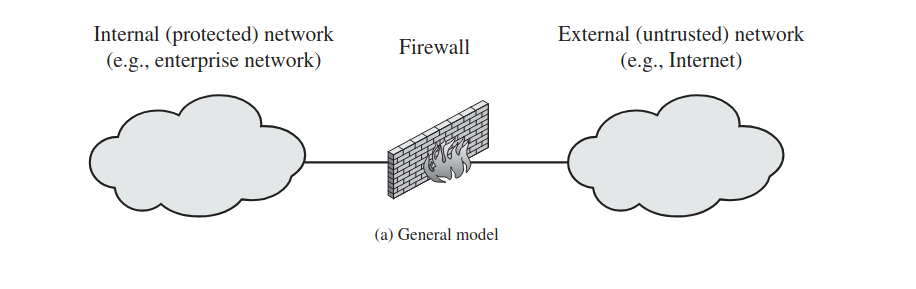
\includegraphics[width=\textwidth]{Figuras/firewall1.png}


    \end{figure}

\end{frame}

\begin{frame}{Tipos de Firewalls}


    \begin{figure}
        \centering
        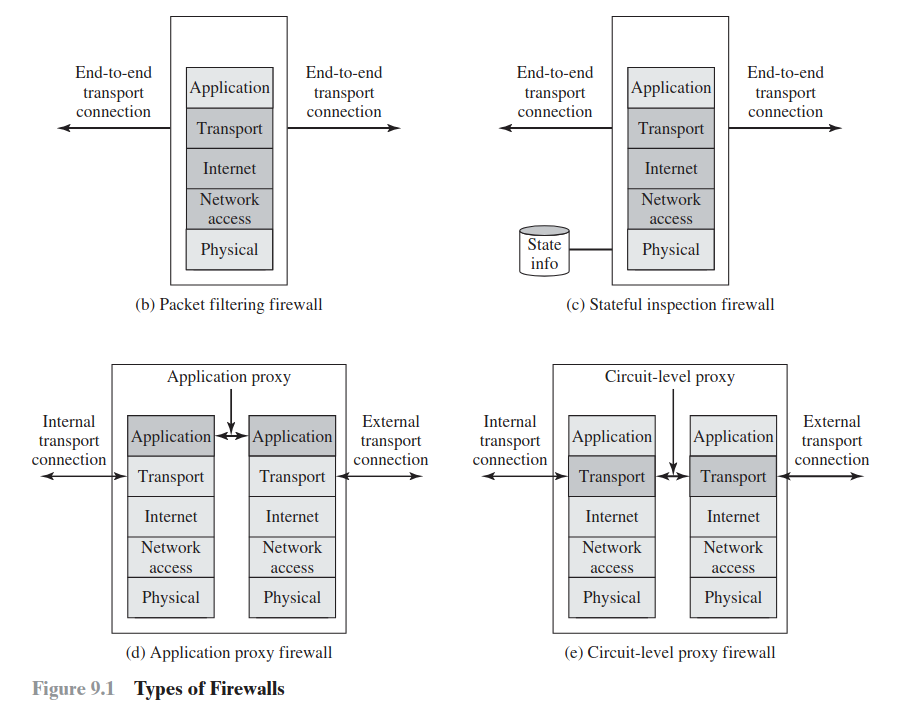
\includegraphics[width=0.7\textwidth]{Figuras/firewall-tipos.png}


    \end{figure}

\end{frame}

\begin{frame}{Introdução: Tipos de Firewalls}
    \begin{itemize}
        \item Um firewall pode monitorar o tráfego de rede em \textbf{vários níveis}:
              \begin{itemize}
                  \item Pacotes de rede de baixo nível (individualmente ou como um fluxo).
                  \item Todo o tráfego dentro de uma conexão de transporte.
                  \item Detalhes dos protocolos de aplicação.
              \end{itemize}

        \item O nível de monitoramento apropriado é determinado pela \textbf{política de acesso} (access policy) desejada.

        \item \textbf{Lógica de Filtragem (Implementa a Política):}
              \begin{itemize}
                  \item \textbf{Filtro Positivo (Positive Filter):} Permite passar \textit{apenas} os pacotes que atendem a critérios específicos.
                  \item \textbf{Filtro Negativo (Negative Filter):} Rejeita \textit{qualquer} pacote que atenda a certos critérios.
              \end{itemize}

        \item \textbf{O que o Firewall Examina (Depende do Tipo):}
              \begin{itemize}
                  \item Um ou mais cabeçalhos de protocolo em cada pacote.
                  \item O \textit{payload} (carga útil) de cada pacote.
                  \item O padrão gerado por uma \textbf{sequência} de pacotes.
              \end{itemize}


    \end{itemize}
\end{frame}

\begin{frame}{Tipo 1: Firewall de Filtro de Pacotes (Definição)}
    \begin{itemize}
        \item Chamado de \textit{Packet Filtering Firewall}.
        \item Aplica um conjunto de regras a \textbf{cada} pacote IP (de entrada e saída).
        \item Ação resultante: \textbf{Encaminhar} (forward) ou \textbf{Descartar} (discard) o pacote.
        \item Tipicamente configurado para filtrar pacotes em \textbf{ambas as direções} (de e para a rede interna).

        \item \textbf{Regras baseadas nas informações do pacote (Camadas 3 e 4):}
              \begin{itemize}
                  \item \textbf{Endereço IP de Origem:} O IP do sistema que originou o pacote.
                  \item \textbf{Endereço IP de Destino:} O IP do sistema que o pacote tenta alcançar.
                  \item \textbf{Porta de Origem/Destino (Nível Transporte):} O número da porta TCP ou UDP (que define aplicações como SNMP ou HTTP).
                  \item \textbf{Campo Protocolo IP:} Define o protocolo de transporte (ex: TCP, UDP, ICMP).
                  \item \textbf{Interface:} Em firewalls com 3+ portas, indica de qual interface o pacote veio ou para qual vai.
              \end{itemize}
    \end{itemize}
\end{frame}

\begin{frame}{Filtro de Pacotes: Lógica de Regras e Políticas Padrão}
    \begin{itemize}
        \item O filtro é configurado como uma \textbf{lista de regras}.
        \item O firewall compara os cabeçalhos (IP/TCP) de cada pacote com esta lista.

        \item \textbf{Se houver correspondência:} A regra é invocada (encaminhar/descartar).
        \item \textbf{Se NÃO houver correspondência:} A \textbf{ação padrão} (default action) é tomada.

        \item \textbf{Duas Políticas Padrão Possíveis:}

        \item \textbf{1. Padrão = Descartar (Default Discard)}
              \begin{itemize}
                  \item "Aquilo que não é expressamente permitido é proibido."
                  \item \textbf{Mais conservadora (segura).}
                  \item Inicialmente, tudo é bloqueado; serviços são adicionados caso a caso.
                  \item Mais visível para usuários (visto como um obstáculo no início).
                  \item Preferida por empresas e governo.
              \end{itemize}

        \item \textbf{2. Padrão = Encaminhar (Default Forward)}
              \begin{itemize}
                  \item "Aquilo que não é expressamente proibido é permitido."
                  \item Aumenta a facilidade de uso para os usuários finais.
                  \item \textbf{Segurança reduzida.}
                  \item O admin deve "reagir" a cada nova ameaça conforme ela se torna conhecida.
                  \item Usada por organizações mais abertas (ex: universidades).
              \end{itemize}
    \end{itemize}
\end{frame}

\begin{frame}{Exemplo de regras de filtragem em Firewalls}


    \begin{figure}
        \centering
        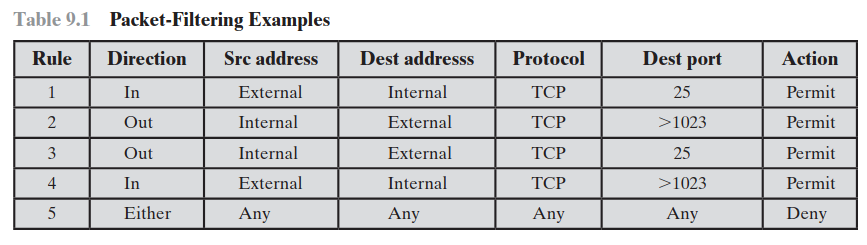
\includegraphics[width=\textwidth]{Figuras/filtragem-de-pacotes.png}


    \end{figure}

\end{frame}

\begin{frame}{Filtro de Pacotes: Exemplo de Regras SMTP (Tabela 9.1)}
    \begin{itemize}
        \item \textbf{Objetivo:} Permitir tráfego de e-mail (SMTP, porta 25) de entrada e saída, mas bloquear todo o resto.
        \item \textbf{Lógica:} Regras aplicadas de cima para baixo (top-to-bottom).

        \item \textbf{Intenção das Regras:}
              \begin{itemize}
                  \item \textbf{Regra 1:} Permitir e-mail \textbf{de entrada} (destino porta 25).
                  \item \textbf{Regra 2:} Permitir a \textbf{resposta} ao e-mail de entrada.
                  \item \textbf{Regra 3:} Permitir e-mail \textbf{de saída} (destino porta 25).
                  \item \textbf{Regra 4:} Permitir a \textbf{resposta} ao e-mail de saída.
                  \item \textbf{Regra 5:} Política padrão (Default = Discard). (Sempre a última regra, explícita ou implicitamente).
              \end{itemize}

        \item \textbf{O Problema (A Falha):}
              \begin{itemize}
                  \item \textbf{A Regra 4 é muito permissiva.} Ela permite tráfego externo para \textbf{qualquer} porta de destino acima de 1023 (assumindo que seja uma "resposta").
              \end{itemize}
    \end{itemize}
\end{frame}

\begin{frame}{Exemplo SMTP: O Exploit e a Solução}
    \begin{itemize}
        \item \textbf{Exemplo de Exploit (usando a Regra 4):}
              \begin{itemize}
                  \item Um atacante externo abre uma conexão da porta 5150 (do atacante) para um Web Proxy interno na porta 8080.
                  \item A Regra 4 (antiga) \textbf{permite} isso, pois a porta de destino (8080) é \> 1023.
                  \item Isso deveria ser proibido e poderia permitir um ataque ao servidor proxy.
              \end{itemize}

        \item \textbf{A Solução (Refinando as Regras):}
              \begin{itemize}
                  \item Configurar o campo de \textbf{porta de origem (source port)} nas regras, tornando-as mais específicas (menos permissivas).
              \end{itemize}

        \item \textbf{Regras Refinadas:}
              \begin{itemize}
                  \item \textbf{Regras 2 e 4 (Respostas):}
                        \begin{itemize}
                            \item Definir a Porta de Origem = \textbf{25}.
                            \item (Pois a resposta a um e-mail deve vir da porta 25 do servidor).
                        \end{itemize}
                  \item \textbf{Regras 1 e 3 (Novas conexões):}
                        \begin{itemize}
                            \item Definir a Porta de Origem = \textbf{\> 1023}.
                            \item (Pois um cliente iniciando um e-mail usará uma porta alta).
                        \end{itemize}
              \end{itemize}
    \end{itemize}
\end{frame}

\begin{frame}{Filtro de Pacotes: Vulnerabilidade Remanescente (SMTP)}
    \begin{itemize}
        \item Mesmo com as regras de porta de origem refinadas, uma vulnerabilidade permanece.

        \item \textbf{A Situação (Regras 3 e 4):}
              \begin{itemize}
                  \item Permitem que qualquer host interno envie e-mail para fora (Porta de Destino = 25).
              \end{itemize}

        \item \textbf{O Problema:}
              \begin{itemize}
                  \item O uso da porta 25 para recebimento de SMTP é apenas um \textbf{padrão} (default).
              \end{itemize}

        \item \textbf{O Risco (O Exploit):}
              \begin{itemize}
                  \item Uma máquina externa (atacante) poderia ser configurada para rodar \textbf{outra aplicação} (maliciosa) na porta 25.
                  \item O atacante poderia então enviar pacotes \textbf{DA} sua porta de origem 25 (TCP Source Port = 25) para tentar invadir máquinas internas.
                  \item A Regra 4 (revisada) permitiria isso, pois ela está configurada para aceitar pacotes \textit{vindos} da porta 25 (assumindo ser uma resposta).
              \end{itemize}
    \end{itemize}
\end{frame}

\begin{frame}{Filtro de Pacotes: A Solução (Flag ACK)}
    \begin{itemize}
        \item \textbf{A Contramedida:}
              \begin{itemize}
                  \item Para combater essa ameaça, podemos adicionar um campo de \textbf{Flag ACK} (ACK flag) à verificação da regra.
              \end{itemize}

        \item \textbf{Onde aplicar:}
              \begin{itemize}
                  \item Esta verificação é adicionada à \textbf{Regra 4} (a regra que permite a \textit{resposta} do servidor externo).
              \end{itemize}

        \item \textbf{A Nova Lógica (Regra 4):}
              \begin{itemize}
                  \item A regra agora exigiria que o \textbf{flag ACK} esteja \textbf{definido} (set) no pacote de entrada.
              \end{itemize}

        \item \textbf{Por que isso funciona?}
              \begin{itemize}
                  \item Um pacote que é parte de uma conexão TCP \textbf{estabelecida} (como uma resposta SMTP legítima) \textbf{SEMPRE} terá o flag ACK definido.
                  \item Um pacote de um atacante tentando \textbf{iniciar} uma nova conexão (o exploit) \textbf{NÃO} teria o flag ACK definido (ex: teria um flag SYN).
              \end{itemize}

        \item A Regra 4 agora se pareceria com:
              \begin{itemize}
                  \item (O texto a seguir deve descrever a nova regra, incluindo a verificação do Flag ACK).
              \end{itemize}
    \end{itemize}
\end{frame}

\begin{frame}{Exemplo de regras de filtragem em Firewalls}


    \begin{figure}
        \centering
        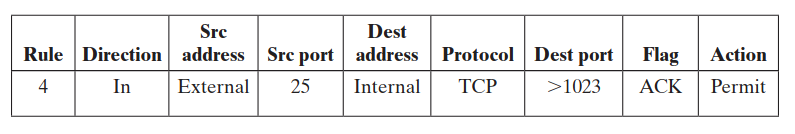
\includegraphics[width=\textwidth]{Figuras/filtro-pacote02.png}


    \end{figure}
    \textbf{A Lógica da Nova Regra:}
    \begin{itemize}
        \item A regra agora permite pacotes de entrada (respostas) que possuem:
              \begin{itemize}
                  \item Porta de Origem (Source Port) = 25
                  \item \textbf{E} o flag ACK definido no segmento TCP.
              \end{itemize}
        \item (Isso efetivamente bloqueia pacotes que \textit{iniciam} conexões (ex: flag SYN) da porta 25, que era a vulnerabilidade.)
    \end{itemize}
\end{frame}

\begin{frame}{Filtro de Pacotes: Vantagens}
    \begin{itemize}
        \item \textbf{1. Simplicidade}
              \begin{itemize}
                  \item A sua lógica de regras é direta (baseada em cabeçalhos L3/L4).
              \end{itemize}

        \item \textbf{2. Transparência}
              \begin{itemize}
                  \item Geralmente são transparentes para os usuários (não exigem configuração no cliente).
              \end{itemize}

        \item \textbf{3. Velocidade}
              \begin{itemize}
                  \item São muito rápidos, pois não inspecionam o payload (carga útil) do pacote.
              \end{itemize}

        \item \textbf{Desvantagens:}
              \begin{itemize}
                  \item O NIST SP 800-41 lista várias fraquezas significativas.
              \end{itemize}
    \end{itemize}
\end{frame}

\begin{frame}{Filtro de Pacotes: Fraquezas (NIST SP 800-41) - Parte 1}
    \begin{itemize}
        \item \textbf{1. Não examina dados da camada superior (Payload)}
              \begin{itemize}
                  \item \textbf{Problema:} Não pode prevenir ataques que usam vulnerabilidades \textbf{específicas da aplicação}.
                  \item \textbf{Exemplo:} Não pode bloquear comandos de aplicação específicos (se o firewall permite a aplicação, todas as funções dela são permitidas).
              \end{itemize}

        \item \textbf{2. Funcionalidade de Log Limitada}
              \begin{itemize}
                  \item \textbf{Problema:} Devido à informação limitada que o firewall vê.
                  \item \textbf{Conteúdo do Log:} Geralmente contém apenas as informações usadas para a decisão (IPs de origem/destino, tipo de tráfego).
              \end{itemize}
    \end{itemize}
\end{frame}

\begin{frame}{Filtro de Pacotes: Fraquezas (NIST SP 800-41) - Parte 2}
    \begin{itemize}
        \item \textbf{3. Não suporta autenticação avançada de usuário}
              \begin{itemize}
                  \item \textbf{Problema:} Novamente, devido à falta de funcionalidade de camada superior.
              \end{itemize}

        \item \textbf{4. Vulnerável a ataques contra a pilha TCP/IP}
              \begin{itemize}
                  \item \textbf{Exemplo:} \textit{Network layer address spoofing} (falsificação de endereço IP).
                  \item \textbf{Problema:} Muitos filtros não conseguem detectar um pacote onde a informação de endereçamento (Camada 3) foi alterada.
                  \item \textbf{Uso:} Usado por intrusos para "burlar" (bypass) os controles do firewall.
              \end{itemize}

        \item \textbf{5. Suscetível a configurações incorretas (Misconfiguration)}
              \begin{itemize}
                  \item \textbf{Problema:} Devido ao pequeno número de variáveis usadas nas decisões.
                  \item \textbf{Risco:} É fácil configurar acidentalmente o firewall para permitir tráfego que deveria ser negado.
              \end{itemize}
    \end{itemize}
\end{frame}

\begin{frame}{Ataques ao Filtro de Pacotes: IP Address Spoofing}
    \begin{itemize}
        \item \textbf{O Ataque (IP Address Spoofing):}
              \begin{itemize}
                  \item O intruso transmite pacotes \textbf{de fora} da rede.
                  \item O campo "Source IP Address" (IP de Origem) é falsificado (spoofed) para conter o endereço de um \textbf{host interno} confiável.
              \end{itemize}

        \item \textbf{O Objetivo:}
              \begin{itemize}
                  \item Penetrar sistemas que empregam segurança simples baseada no endereço de origem (ex: "aceitar pacotes vindos de IPs internos confiáveis").
              \end{itemize}

        \item \textbf{A Contramedida:}
              \begin{itemize}
                  \item O firewall (ou roteador externo) deve \textbf{descartar} pacotes se:
                        \begin{itemize}
                            \item O pacote chega na interface \textbf{externa}.
                            \item \textbf{E} o pacote possui um endereço de origem (source address) \textbf{interno}.
                        \end{itemize}
              \end{itemize}
    \end{itemize}
\end{frame}



\begin{frame}{Ataques ao Filtro de Pacotes: Tiny Fragment}
    \begin{itemize}
        \item \textbf{O Ataque (Tiny Fragment Attack):}
              \begin{itemize}
                  \item O intruso usa a opção de fragmentação IP para criar \textbf{fragmentos extremamente pequenos}.
                  \item \textbf{Objetivo:} Forçar o cabeçalho TCP (que contém as portas) para um \textbf{fragmento separado} (ex: o segundo fragmento), deixando o primeiro fragmento apenas com o cabeçalho IP.
              \end{itemize}

        \item \textbf{A Lógica do Ataque:}
              \begin{itemize}
                  \item O filtro de pacotes toma sua decisão (Permitir/Negar) com base no \textbf{primeiro fragmento}.
                  \item O atacante espera que o primeiro fragmento (incompleto) seja permitido, e que os fragmentos subsequentes (com o TCP malicioso) passem direto.
              \end{itemize}

        \item \textbf{A Contramedida:}
              \begin{itemize}
                  \item Reforçar uma regra de que o \textbf{primeiro fragmento} de um pacote \textbf{deve conter} uma quantidade mínima predefinida do cabeçalho de transporte (TCP).
                  \item (Se o primeiro fragmento for rejeitado, o filtro deve memorizar o ID do pacote e descartar todos os fragmentos subsequentes).
              \end{itemize}
    \end{itemize}
\end{frame}

\begin{frame}{O Problema do Filtro de Pacotes (Falta de Contexto)}
    \begin{itemize}
        \item Um filtro de pacotes tradicional (stateless) toma decisões \textbf{pacote a pacote}.
        \item Ele \textbf{não considera o contexto} de camada superior (se uma conexão TCP existe).

        \item \textbf{Contexto (Modelo Cliente/Servidor):}
              \begin{itemize}
                  \item Aplicações (ex: SMTP) usam TCP.
                  \item \textbf{Servidor (ex: SMTP):} Usa uma "porta bem conhecida" (well-known), que é fixa e < 1024 (ex: Porta \textbf{25}).
                  \item \textbf{Cliente (ex: usuário):} Usa uma porta dinâmica, temporária e > 1024 (ex: Porta \textbf{49152}).
              \end{itemize}

        \item \textbf{A Vulnerabilidade do Filtro de Pacotes:}
              \begin{itemize}
                  \item Para permitir o tráfego de \textit{resposta} (do servidor na porta 25 para o cliente na porta 49152), o firewall deve permitir tráfego de entrada em \textbf{TODAS} as portas altas (>1023).
                  \item Isso cria uma vulnerabilidade enorme que pode ser explorada por atacantes.
              \end{itemize}
    \end{itemize}
\end{frame}

\begin{frame}{Tipo 2: Firewall de Inspeção de Estado (Stateful)}
    \begin{itemize}
        \item (Stateful Packet Inspection Firewall).
        \item \textbf{A Solução:} "Aperta" as regras para o tráfego TCP.

        \item \textbf{O Mecanismo (O "Estado"):}
              \begin{itemize}
                  \item O firewall cria e mantém um \textbf{diretório (Tabela de Estado)} das conexões TCP de \textit{saída} (outbound) que estão ativas.
                  \item (Ref: Tabela 9.2).
                  \item Uma entrada é criada para cada conexão atualmente estabelecida.
              \end{itemize}

        \item \textbf{A Nova Lógica de Filtragem:}
              \begin{itemize}
                  \item O firewall agora permite tráfego de entrada em portas altas (>1023) \textbf{APENAS} se este pacote \textbf{corresponder} (fit the profile) a uma das entradas (conexões) existentes no diretório (Tabela de Estado).
              \end{itemize}
    \end{itemize}
\end{frame}

\begin{frame}{Firewall de Inspeção de Estado (Capacidades)}
    \begin{itemize}
        \item Um firewall stateful revisa as mesmas informações que um filtro de pacotes (cabeçalhos L3/L4).

        \item \textbf{MAS TAMBÉM...}
              \begin{itemize}
                  \item Registra informações sobre o \textbf{estado da conexão TCP} (ex: estabelecida, fechando, etc.).
              \end{itemize}

        \item \textbf{Recursos Avançados (em alguns firewalls stateful):}
              \begin{itemize}
                  \item \textbf{Rastreamento de Números de Sequência TCP:}
                        \begin{itemize}
                            \item Usado para prevenir ataques que dependem do número de sequência (ex: \textit{session hijacking}).
                        \end{itemize}
                  \item \textbf{Inspeção Limitada de Aplicação (Deep Packet Inspection - DPI):}
                        \begin{itemize}
                            \item Inspecionam (de forma limitada) os dados da aplicação.
                            \item Útil para protocolos "problemáticos" (ex: FTP, IM, SIPS) para identificar e rastrear conexões de dados relacionadas.
                        \end{itemize}
              \end{itemize}
    \end{itemize}
\end{frame}

\begin{frame}{Filtro de pacotes com estado}


    \begin{figure}
        \centering
        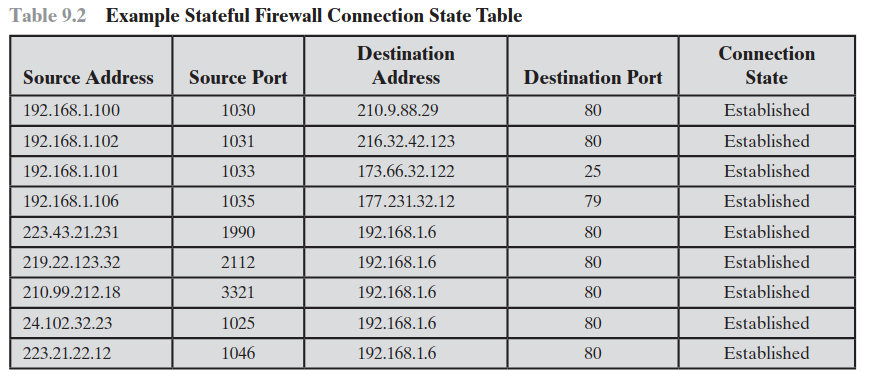
\includegraphics[width=\textwidth]{Figuras/firewall-filtro-de-pacotes-stateful.png}


    \end{figure}

\end{frame}

\begin{frame}{Tipo 3: Application-Level Gateway (Proxy de Aplicação)}
    \begin{itemize}
        \item Também chamado de \textbf{Application Proxy}.
        \item Atua como um \textbf{"relay" (retransmissor)} do tráfego em nível de aplicação (ex: Telnet, FTP).

        \item \textbf{Mecanismo de "Dupla Conexão" (Splice):}
              \begin{itemize}
                  \item O usuário contata o gateway (proxy).
                  \item O gateway solicita ao usuário o host remoto e as credenciais (ID/autenticação).
                  \item \textbf{Se válido:} O gateway (ele mesmo) contata a aplicação no host remoto.
                  \item O gateway retransmite (relays) os segmentos TCP (dados da aplicação) entre os dois \textit{endpoints}.
                  \item (Existem duas conexões "emendadas" (spliced): Cliente $\leftrightarrow$ Gateway e Gateway $\leftrightarrow$ Servidor).
              \end{itemize}
    \end{itemize}
\end{frame}

\begin{frame}{Application-Level Gateway: Vantagens e Desvantagens}
    \begin{itemize}
        \item \textbf{Controle Granular:}
              \begin{itemize}
                  \item Se o gateway não implementa o código proxy para uma aplicação, o serviço \textbf{não é suportado}.
                  \item Pode ser configurado para suportar apenas \textbf{recursos específicos} de uma aplicação (ex: permitir \texttt{GET} no HTTP, mas negar \texttt{POST}) que o admin considera aceitáveis.
              \end{itemize}

        \item \textbf{Vantagem: Mais Seguro que Filtros de Pacote}
              \begin{itemize}
                  \item Precisa apenas analisar \textbf{algumas aplicações permitidas}, em vez de inúmeras combinações complexas de IP/Porta/Flags.
              \end{itemize}

        \item \textbf{Vantagem: Auditoria (Logging)}
              \begin{itemize}
                  \item É fácil registrar e auditar todo o tráfego no nível da aplicação.
              \end{itemize}

        \item \textbf{Desvantagem: Sobrecarga de Processamento (Overhead)}
              \begin{itemize}
                  \item O gateway deve examinar e encaminhar todo o tráfego nas duas conexões "emendadas".
              \end{itemize}
    \end{itemize}
\end{frame}

\begin{frame}{Tipo 4: Circuit-Level Gateway (Proxy de Circuito)}
    \begin{itemize}
        \item Pode ser um sistema autônomo (stand-alone) ou uma \textbf{função especializada} de um Application-Level Gateway.

        \item \textbf{Mecanismo (Similar ao Proxy de Aplicação):}
              \begin{itemize}
                  \item \textbf{NÃO} permite uma conexão TCP ponta-a-ponta (end-to-end).
                  \item O gateway estabelece \textbf{duas conexões TCP}:
                        \begin{itemize}
                            \item 1. (Host Interno $\leftrightarrow$ Gateway)
                            \item 2. (Gateway $\leftrightarrow$ Host Externo)
                        \end{itemize}
              \end{itemize}

        \item \textbf{Diferença Chave (vs. Application Proxy):}
              \begin{itemize}
                  \item Uma vez estabelecidas as conexões, o gateway retransmite (relays) os segmentos TCP \textbf{sem examinar o conteúdo (payload)}.
                  \item A \textbf{função de segurança} consiste \textit{apenas} em determinar quais conexões serão permitidas.
              \end{itemize}

        \item \textbf{Caso de Uso Típico (Híbrido):}
              \begin{itemize}
                  \item Quando o admin \textbf{confia} nos usuários internos.
                  \item \textit{Inbound (Entrada):} Usa-se Application Proxy (caro, mas seguro).
                  \item \textit{Outbound (Saída):} Usa-se Circuit-Level (barato), pois não se gasta processamento examinando os dados de saída.
              \end{itemize}
    \end{itemize}
\end{frame}

\begin{frame}{Exemplo de Circuit-Level: SOCKS (RFC 1928)}
    \begin{itemize}
        \item SOCKS (versão 5, RFC 1928) é uma implementação de um Circuit-Level Gateway.

        \item \textbf{Definição (RFC):} Um framework para aplicações cliente-servidor (TCP e UDP) usarem os serviços de um firewall de forma conveniente e segura.

        \item \textbf{Posição na Pilha:}
              \begin{itemize}
                  \item É conceitualmente uma "camada de ajuste" (\textit{shim-layer}).
                  \item Fica \textbf{entre} a camada de Aplicação e a camada de Transporte.
                  \item (Não é um gateway de camada de Rede; não encaminha ICMP).
              \end{itemize}

        \item \textbf{Componentes do SOCKS:}
              \begin{itemize}
                  \item \textbf{SOCKS Server:} Roda no firewall (ex: UNIX, Windows).
                  \item \textbf{SOCKS Client Library:} Roda nos hosts internos (protegidos).
                  \item \textbf{Clientes "SOCKS-ificados":} Programas (FTP, TELNET) recompilados ou "relinkados" para usar a biblioteca SOCKS.
              \end{itemize}
    \end{itemize}
\end{frame}

\begin{frame}{SOCKS: Mecanismo de Operação (TCP e UDP)}
    \begin{itemize}
        \item \textbf{Fluxo de Conexão TCP:}
              \begin{itemize}
                  \item 1. O cliente (interno) abre uma conexão TCP com o \textbf{Servidor SOCKS} (na porta TCP \textbf{1080}).
                  \item 2. O cliente negocia o método de autenticação.
                  \item 3. O cliente se autentica.
                  \item 4. O cliente envia uma \textbf{solicitação de relay} (relay request) (ex: "quero conectar no IP 1.2.3.4, porta 80").
                  \item 5. O Servidor SOCKS avalia o pedido e (se permitido) estabelece a conexão externa.
              \end{itemize}

        \item \textbf{Tratamento de UDP (Similar):}
              \begin{itemize}
                  \item Uma conexão \textbf{TCP} é aberta primeiro (para o SOCKS, porta 1080) apenas para \textbf{autenticar} o usuário.
                  \item Os segmentos UDP são então encaminhados (relay) pelo firewall \textit{enquanto} essa conexão TCP de controle permanecer aberta.
              \end{itemize}
    \end{itemize}
\end{frame}

\begin{frame}{9.4 Plataformas de Firewall (Firewall Basing)}
    \begin{itemize}
        \item É comum instalar um firewall em uma \textbf{máquina "stand-alone"} (dedicada).
              \begin{itemize}
                  \item Rodando um S.O. comum (ex: UNIX, Linux).
                  \item \textbf{Ou que} ... Pode ser fornecido como um "security appliance" pré-configurado.
              \end{itemize}

        \item \textbf{Alternativas:}
              \begin{itemize}
                  \item A funcionalidade de firewall também pode ser implementada como um \textbf{módulo de software} em:
                        \begin{itemize}
                            \item Um Roteador.
                            \item Um Switch LAN.
                            \item Um Servidor.
                        \end{itemize}
              \end{itemize}

        \item Esta seção analisa considerações adicionais sobre essas plataformas.
    \end{itemize}
\end{frame}

\begin{frame}{Host Bastião: Definição}
    \begin{itemize}
        \item Um \textbf{Host Bastião} é um sistema identificado pelo administrador do firewall como um \textbf{"ponto forte crítico"} (critical strong point) na segurança da rede.

        \item \textbf{Função Típica:}
              \begin{itemize}
                  \item Serve como plataforma para \textbf{Gateways} (de Nível de Aplicação ou Nível de Circuito).
                  \item Pode suportar outros serviços (ex: IPsec).
              \end{itemize}

        \item \textbf{Característica Principal:}
              \begin{itemize}
                  \item A plataforma de hardware executa uma \textbf{versão segura} do seu S.O.
                  \item Isso o torna um \textbf{Sistema Reforçado} (Hardened System).
              \end{itemize}
    \end{itemize}
\end{frame}

\begin{frame}{Características do Host Bastião (Parte 1: Hardening e Acesso)}
    \begin{itemize}
        \item \textbf{Serviços Mínimos:}
              \begin{itemize}
                  \item \textbf{Apenas} os serviços que o administrador considera \textbf{essenciais} são instalados.
                  \item Ex: Proxies para DNS, FTP, HTTP, SMTP.
              \end{itemize}

        \item \textbf{Autenticação Adicional:}
              \begin{itemize}
                  \item O host pode exigir \textbf{autenticação extra} antes de permitir o acesso aos serviços de proxy.
                  \item Além disso, cada serviço de proxy (individualmente) pode exigir sua própria autenticação.
              \end{itemize}
    \end{itemize}
\end{frame}

\begin{frame}{Características do Host Bastião (Parte 2: Restrições de Proxy)}
    \begin{itemize}
        \item \textbf{Subconjunto de Comandos (Command Subset):}
              \begin{itemize}
                  \item Cada proxy é configurado para suportar apenas um \textbf{subconjunto} dos comandos padrão da aplicação (ex: bloquear certas funções do HTTP).
              \end{itemize}

        \item \textbf{Acesso Restrito a Hosts:}
              \begin{itemize}
                  \item Cada proxy é configurado para permitir acesso \textbf{apenas a sistemas host específicos} (internos).
              \end{itemize}

        \item \textbf{Auditoria Detalhada (Logging):}
              \begin{itemize}
                  \item Cada proxy mantém logs de auditoria detalhados (todo o tráfego, cada conexão, duração).
                  \item (Ferramenta essencial para descobrir e terminar ataques).
              \end{itemize}
    \end{itemize}
\end{frame}

\begin{frame}{Características do Host Bastião (Parte 3: Design de Software)}
    \begin{itemize}
        \item \textbf{Simplicidade do Software:}
              \begin{itemize}
                  \item Cada proxy é um pacote de software \textbf{muito pequeno}, desenhado especificamente para segurança.
                  \item \textbf{Vantagem:} Mais fácil de verificar (auditar) em busca de falhas de segurança.
                  \item \textit{Ex: App de e-mail UNIX (20.000+ linhas) vs. Proxy de e-mail (< 1.000 linhas).}
              \end{itemize}

        \item \textbf{Independência (Modularidade):}
              \begin{itemize}
                  \item Cada proxy é \textbf{independente} dos outros no host.
                  \item \textbf{Vantagem:} Se um proxy tiver uma vulnerabilidade, ele pode ser desinstalado sem afetar os outros.
                  \item \textbf{Vantagem:} Fácil de adicionar suporte a novos serviços instalando um novo proxy.
              \end{itemize}
    \end{itemize}
\end{frame}

\begin{frame}{Características do Host Bastião (Parte 4: Segurança em Runtime)}
    \begin{itemize}
        \item \textbf{Sem Acesso a Disco:}
              \begin{itemize}
                  \item Um proxy (geralmente) não realiza acesso a disco, exceto para ler seu arquivo de configuração inicial.
                  \item \textbf{Vantagem:} As partes do sistema de arquivos com código executável podem ser tornadas \textbf{somente-leitura}.
                  \item \textbf{Resultado:} Dificulta para um intruso instalar \textit{Trojan horses}, \textit{sniffers} ou outros arquivos.
              \end{itemize}

        \item \textbf{Sem Privilégios:}
              \begin{itemize}
                  \item Cada proxy roda como um \textbf{usuário não-privilegiado} (nonprivileged user).
                  \item Roda em um diretório privado e seguro no host bastião.
              \end{itemize}
    \end{itemize}
\end{frame}
\begin{frame}{Host-Based Firewalls }
    \begin{itemize}
        \item \textbf{O que é?}
              \begin{itemize}
                  \item Um \textbf{módulo de software} usado para proteger um \textbf{host individual}.
                  \item Disponível no S.O. ou como pacote add-on.
                  \item Filtra e restringe o fluxo de pacotes (assim como firewalls stand-alone).
                  \item Localização comum: em um \textbf{servidor}.
              \end{itemize}

        \item \textbf{Vantagens:}
              \begin{itemize}
                  \item \textbf{1. Regras Personalizadas:}
                        \begin{itemize}
                            \item As regras de filtragem podem ser adaptadas ao ambiente específico do host (ex: filtros diferentes para servidores de aplicações diferentes).
                        \end{itemize}
                  \item \textbf{2. Proteção Independente da Topologia:}
                        \begin{itemize}
                            \item Ataques \textbf{internos} e externos devem passar pelo firewall do host.
                        \end{itemize}
                  \item \textbf{3. Camada Adicional de Proteção:}
                        \begin{itemize}
                            \item Usado \textit{em conjunto} com firewalls stand-alone (defesa em profundidade).
                            \item Permite adicionar novos servidores à rede (com seus próprios firewalls) sem a necessidade de alterar a configuração do firewall da rede.
                        \end{itemize}
              \end{itemize}
    \end{itemize}
\end{frame}

\begin{frame}{Firewalls em Dispositivos de Rede}
    \begin{itemize}
        \item \textbf{O que são?}
              \begin{itemize}
                  \item Funcionalidades de firewall (especialmente filtro de pacotes e stateful inspection) implementadas diretamente em dispositivos de rede.
              \end{itemize}

        \item \textbf{Onde?}
              \begin{itemize}
                  \item Comumente em \textbf{roteadores} e \textbf{switches}.
              \end{itemize}

        \item \textbf{Função:}
              \begin{itemize}
                  \item Monitorar e filtrar os fluxos de pacotes que passam \textit{através} do dispositivo.
              \end{itemize}

        \item \textbf{Propósito (Defesa em Profundidade):}
              \begin{itemize}
                  \item Usados para fornecer \textbf{camadas adicionais de proteção}, em conjunto com bastion hosts e host-based firewalls.
              \end{itemize}
    \end{itemize}
\end{frame}

\begin{frame}{Virtual Firewalls (Firewalls Virtuais)}
    \begin{itemize}
        \item \textbf{Contexto: Ambientes Virtualizados}
              \begin{itemize}
                  \item Em vez de dispositivos físicos separados (servidores, switches, firewalls), usam-se versões \textbf{virtualizadas} que compartilham o mesmo hardware físico.
              \end{itemize}

        \item \textbf{Implementações (Duas Formas):}
              \begin{itemize}
                  \item \textbf{1. Appliance Virtual:} Pode ser um "bastion host" virtualizado (rodando como uma VM).
                  \item \textbf{2. No Hypervisor:} As capacidades de firewall podem ser fornecidas diretamente pelo \textbf{hypervisor} (o software que gerencia as máquinas virtuais).
              \end{itemize}
    \end{itemize}
\end{frame}

\begin{frame}{Locais de um firewall}


    \begin{figure}
        \centering
        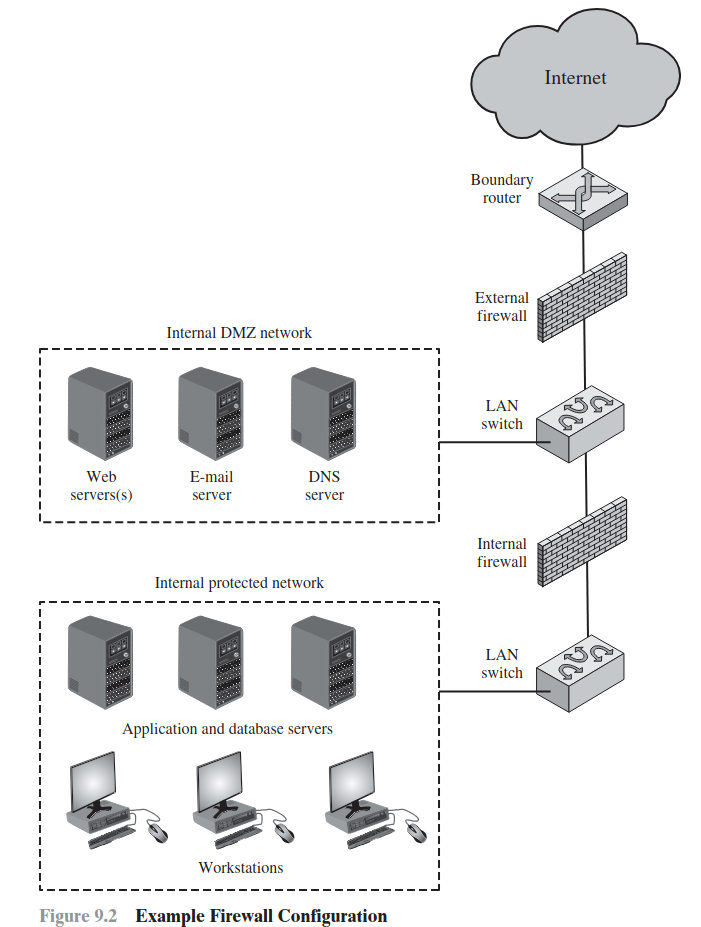
\includegraphics[width=0.4\textwidth]{Figuras/firewall-locations.png}


    \end{figure}

\end{frame}

\begin{frame}{Firewalls em dispositivos locais: Definição}
    \begin{itemize}
        \item \textbf{O que é?}
              \begin{itemize}
                  \item Controla o tráfego entre um \textbf{computador pessoal} (ou workstation) e a rede (Internet ou rede corporativa).
              \end{itemize}

        \item \textbf{Casos de Uso:}
              \begin{itemize}
                  \item Ambiente doméstico (home).
                  \item Intranets corporativas.
              \end{itemize}

        \item \textbf{Localização (Implementação):}
              \begin{itemize}
                  \item \textbf{1. Módulo de Software:} Tipicamente, roda no próprio computador pessoal.
                  \item \textbf{2. Roteador Doméstico:} Em ambientes com múltiplos computadores, a funcionalidade pode estar no roteador que se conecta ao modem (DSL/Cabo).
              \end{itemize}
    \end{itemize}
\end{frame}

\begin{frame}{Firewalls em dispositivos locais: Função e Implementações}
    \begin{itemize}
        \item \textbf{Complexidade:}
              \begin{itemize}
                  \item Tipicamente \textbf{muito menos complexos} que firewalls de servidor ou stand-alone.
              \end{itemize}

        \item \textbf{Função Principal (Defesa):}
              \begin{itemize}
                  \item Negar acesso remoto \textbf{não autorizado} ao computador.
              \end{itemize}

        \item \textbf{Função Secundária (Detecção):}
              \begin{itemize}
                  \item Monitorar atividade \textbf{de saída} (outgoing) na tentativa de detectar e bloquear malware (ex: worms).
              \end{itemize}

        \item \textbf{Implementações (Exemplos):}
              \begin{itemize}
                  \item Pacote \texttt{netfilter} (Linux).
                  \item Pacote \texttt{pf} (BSD e MacOS).
                  \item \texttt{Windows Firewall} (Windows).
              \end{itemize}

        \item \textbf{Configuração:}
              \begin{itemize}
                  \item Via linha de comando (CLI) ou interface gráfica (GUI).
              \end{itemize}
    \end{itemize}
\end{frame}

\begin{frame}{Firewalls em dispositivos locais: Política Padrão e Serviços}
    \begin{itemize}
        \item \textbf{Política Padrão (Default):}
              \begin{itemize}
                  \item \textbf{Conexões de Entrada (Inbound):} Geralmente \textbf{negadas}, exceto as que o usuário permite explicitamente.
                  \item \textbf{Conexões de Saída (Outbound):} Geralmente \textbf{permitidas}.
              \end{itemize}

        \item \textbf{Exemplos de serviços de entrada que podem ser reativados (portas):}
              \begin{columns}[T] % T = top aligned
                  \begin{column}{.5\textwidth}
                      \begin{itemize}
                          \item Personal file sharing (548, 427)
                          \item Windows sharing (139)
                          \item Personal Web sharing (80, 427)
                          \item Remote login—SSH (22)
                          \item FTP access (20-21, etc.)
                          \item Printer sharing (631, 515)
                          \item IChat Rendezvous (5297, 5298)
                          \item iTunes Music Sharing (3869)
                      \end{itemize}
                  \end{column}
                  \begin{column}{.5\textwidth}
                      \begin{itemize}
                          \item CVS (2401)
                          \item Gnutella/Limewire (6346)
                          \item ICQ (4000)
                          \item IRC (194)
                          \item MSN Messenger (6891-6900)
                          \item Network Time (123)
                          \item SMB (sem netbios–445)
                          \item VNC (5900-5902)
                      \end{itemize}
                  \end{column}
              \end{columns}
    \end{itemize}
\end{frame}

\begin{frame}{Firewalls em dispositivos locais: Regra de FTP e Recursos Avançados}
    \begin{itemize}
        \item \textbf{Exceção da Regra de FTP:}
              \begin{itemize}
                  \item Se o acesso FTP é habilitado, as portas 20 e 21 são abertas localmente.
                  \item Se \textit{outros} conectam \textit{a partir} das portas 20 ou 21, as portas 1024-65535 são abertas (para a conexão de dados do FTP).
              \end{itemize}

        \item \textbf{Recursos Avançados:}
              \begin{itemize}
                  \item \textbf{Stealth Mode:} "Esconde" o sistema na Internet ao \textbf{descartar (drop)} pacotes de comunicação não solicitados (fazendo parecer que o sistema não está presente).
                  \item \textbf{Bloqueio de UDP:} Restringe o tráfego (para portas abertas) apenas a pacotes TCP.
                  \item \textbf{Logging:} Ferramenta importante para verificar atividades indesejadas.
                  \item \textbf{Filtro de Aplicação:} Permite ao usuário especificar que \textbf{apenas aplicações selecionadas} (ou assinadas por uma CA válida) podem prover serviços na rede.
              \end{itemize}
    \end{itemize}
\end{frame}

\begin{frame}{9.5 Localização e Configurações do Firewall}
    \begin{itemize}
        \item O firewall é posicionado para prover uma \textbf{barreira protetora} entre uma fonte externa (potencialmente não confiável) e uma rede interna.

        \item O administrador de segurança deve decidir:
              \begin{itemize}
                  \item A \textbf{localização} do firewall.
                  \item O \textbf{número} de firewalls necessários.
              \end{itemize}

        \item Esta seção analisa algumas opções comuns de configuração e localização.
    \end{itemize}
\end{frame}

\begin{frame}{Configuração: Redes DMZ (Zona Desmilitarizada)}
    \begin{itemize}
        \item Uma configuração de firewall comum que inclui um \textbf{segmento de rede adicional} entre um firewall \textbf{externo} e um \textbf{interno}.

        \item \textbf{Firewall Externo:} Colocado na borda da rede (logo após o roteador de borda da Internet/WAN).

        \item \textbf{Firewall(s) Interno(s):} Protegem o grosso da rede corporativa (enterprise network).

        \item \textbf{A DMZ:} É a região (rede) localizada \textit{entre} esses dois firewalls.

        \item \textbf{Propósito da DMZ:}
              \begin{itemize}
                  \item Localizar sistemas que precisam ser \textbf{acessíveis externamente}, mas que ainda necessitam de \textbf{alguma proteção}.
                  \item \textbf{Exemplos de sistemas na DMZ:} Website corporativo, Servidor de e-mail (SMTP), Servidor DNS.
              \end{itemize}
    \end{itemize}
\end{frame}

\begin{frame}{DMZ: O Papel de Cada Firewall}
    \begin{itemize}
        \item \textbf{Função do Firewall Externo:}
              \begin{itemize}
                  \item Fornece controle de acesso e proteção (moderada) para os sistemas da DMZ (consistente com sua necessidade de conectividade).
                  \item Fornece um nível básico de proteção para o resto da rede interna.
              \end{itemize}

        \item \textbf{Três Propósitos do Firewall Interno:}
              \begin{enumerate}
                  \item \textbf{Filtragem mais rigorosa:} Adiciona capacidade de filtragem mais forte (comparado ao externo) para proteger os servidores/workstations internos de ataques externos.

                  \item \textbf{Proteção de Mão Dupla (vs. DMZ):}
                        \begin{itemize}
                            \item Protege a rede interna contra ataques lançados \textit{a partir} da DMZ (ex: se um servidor web for comprometido com malware, rootkits, bots).
                            \item Protege a DMZ contra ataques vindos da rede \textit{interna}.
                        \end{itemize}

                  \item \textbf{Segmentação Interna:}
                        \begin{itemize}
                            \item Múltiplos firewalls internos podem ser usados para proteger porções da rede interna umas das outras (ex: Servidores vs. Workstations, como na Fig 8.5).
                        \end{itemize}
              \end{enumerate}
    \end{itemize}
\end{frame}

\begin{frame}{Configuração: Redes Privadas Virtuais (VPNs)}
    \begin{itemize}
        \item \textbf{O Problema (Custo vs. Segurança):}
              \begin{itemize}
                  \item Organizações (com LANs em locais dispersos) precisam se interconectar.
                  \item Usar a \textbf{Internet} (rede pública) é mais barato e mais fácil de gerenciar (offloading) do que usar uma \textbf{rede privada} (linhas privadas).
                  \item \textbf{Mas:} A rede pública expõe o tráfego corporativo (eavesdropping, acesso não autorizado).
              \end{itemize}

        \item \textbf{A Solução (VPN):}
              \begin{itemize}
                  \item Um conjunto de computadores que se interconecta por uma rede insegura.
                  \item Usa \textbf{criptografia e autenticação} em camadas de protocolo inferiores.
                  \item Cria uma \textbf{conexão segura} através de uma rede insegura (Internet).
                  \item \textit{Pré-requisito:} Depende de ter o mesmo sistema de cripto/autenticação em ambas as pontas.
              \end{itemize}
    \end{itemize}
\end{frame}

\begin{frame}{VPNs: Implementação com IPsec}
    \begin{itemize}
        \item A criptografia pode ser feita pelo \textbf{software do firewall} ou por roteadores.
        \item Protocolo mais comum: \textbf{IPsec} (nível IP).

        \item \textbf{Cenário Típico:}
              \begin{itemize}
                  \item Protocolos IPsec operam em dispositivos de rede (roteador ou firewall) que conectam a LAN ao mundo externo.
                  \item O dispositivo IPsec \textbf{criptografa e comprime} todo o tráfego que \textit{sai} para a WAN.
                  \item O dispositivo IPsec \textbf{descriptografa e descomprime} todo o tráfego que \textit{vem} da WAN.
                  \item Esta operação é \textbf{transparente} para os servidores e workstations na LAN.
              \end{itemize}

        \item \textbf{Usuários Individuais (Remotos):}
              \begin{itemize}
                  \item Também podem usar IPsec, mas o \textit{próprio workstation} deve implementar os protocolos e ter alta segurança de host (tornando-se um alvo atraente).
              \end{itemize}
    \end{itemize}
\end{frame}

\begin{frame}{VPNs: Onde implementar o IPsec?}
    \begin{itemize}
        \item Um local lógico para implementar o IPsec é \textbf{no firewall}.

        \item \textbf{Problema 1: IPsec \textit{atrás} (interno) do firewall}
              \begin{itemize}
                  \item O tráfego VPN que passa pelo firewall (em ambas as direções) está \textbf{criptografado}.
                  \item \textbf{Consequência:} O firewall é \textbf{incapaz} de realizar suas funções (filtragem, scan de vírus, log, controle de acesso, etc.), pois não vê o tráfego em claro.
              \end{itemize}

        \item \textbf{Problema 2: IPsec \textit{no roteador de borda} (externo ao firewall)}
              \begin{itemize}
                  \item O dispositivo (roteador) é provavelmente \textbf{menos seguro} que o firewall.
                  \item Portanto, é uma plataforma menos desejável para o IPsec.
              \end{itemize}

        \item \textit{(Solução implícita: A implementação do IPsec no próprio firewall é a mais funcional).}
    \end{itemize}
\end{frame}

\begin{frame}{Configuração: Firewalls Distribuídos}
    \begin{itemize}
        \item \textbf{O que é?} Uma configuração que envolve:
              \begin{itemize}
                  \item Dispositivos de firewall stand-alone (de rede).
                  \item \textbf{E} Host-Based Firewalls (em servidores, workstations).
              \end{itemize}

        \item \textbf{Característica Chave:} Trabalham juntos sob um \textbf{controle administrativo central}.

        \item \textbf{Gerenciamento:}
              \begin{itemize}
                  \item Administradores configuram firewalls em centenas de servidores/workstations e firewalls pessoais (locais e remotos).
                  \item Ferramentas permitem ao admin definir políticas e monitorar a segurança em \textbf{toda a rede}.
              \end{itemize}

        \item \textbf{Vantagem:}
              \begin{itemize}
                  \item Proteção contra \textbf{ataques internos}.
                  \item Proteção \textbf{personalizada} (tailored) para máquinas e aplicações específicas.
              \end{itemize}
    \end{itemize}
\end{frame}

\begin{frame}{Configuração: Firewalls Distribuídos}
    \begin{itemize}
        \item \textbf{O que é?} Uma configuração que envolve:
              \begin{itemize}
                  \item Dispositivos de firewall stand-alone (de rede).
                  \item \textbf{E} Host-Based Firewalls (em servidores, workstations).
              \end{itemize}

        \item \textbf{Característica Chave:} Trabalham juntos sob um \textbf{controle administrativo central}.

        \item \textbf{Gerenciamento:}
              \begin{itemize}
                  \item Administradores configuram firewalls em centenas de servidores/workstations e firewalls pessoais (locais e remotos).
                  \item Ferramentas permitem ao admin definir políticas e monitorar a segurança em \textbf{toda a rede}.
              \end{itemize}

        \item \textbf{Vantagem:}
              \begin{itemize}
                  \item Proteção contra \textbf{ataques internos}.
                  \item Proteção \textbf{personalizada} (tailored) para máquinas e aplicações específicas.
              \end{itemize}
    \end{itemize}
\end{frame}